\chapter{Atelier de peinture et de polissage}
Passons maintenant à un système composé d'un atelier et d'un robot qui permet de réaliser les actions peinture/polissage pour ensuite déservir les pièces dans un stock. Pour la modélisation des automates At (atelier) et St (stock), nous avons choisi les modèles suivants :
\begin{figure}[!ht]
\begin{minipage}{.5\textwidth}
\centering
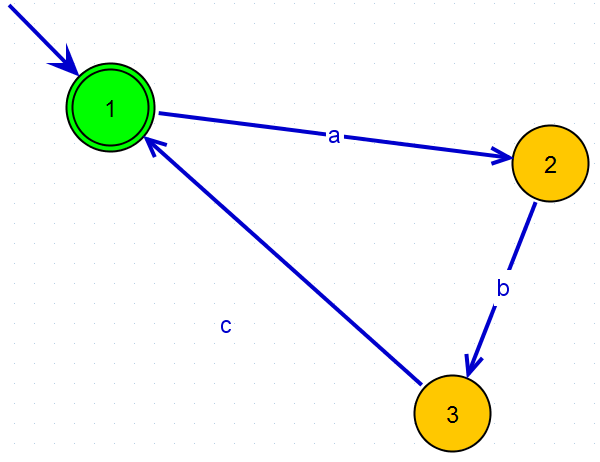
\includegraphics[width=\textwidth]{./II/images/At.png}
\caption{Atelier At}
\end{minipage} \hfill
\begin{minipage}{.5\textwidth}
\centering
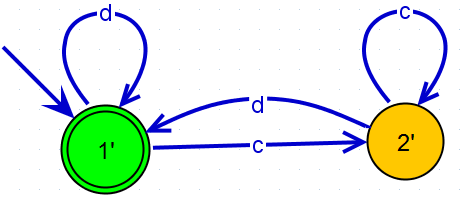
\includegraphics[width=\textwidth]{./II/images/St.png}
\caption{Stock St}
\end{minipage}
\end{figure}

avec pour alphabet de At et St:
\begin{itemize}[label = \textbullet]
\item $\Sigma_{At} = \left\lbrace a,b,c \right\rbrace $
\item $\Sigma_{St} = \left\lbrace c,d\right\rbrace$
\item les évènements non contrôlables sont : $\Sigma_{nc}=\left\lbrace b,c \right\rbrace$, tous les autres évènements sont observables et contrôlables.
\end{itemize}

En utilisant le produit parallèle, nous avons obtenu notre modèle du procédé qui est le suivant : \begin{figure}
\centering
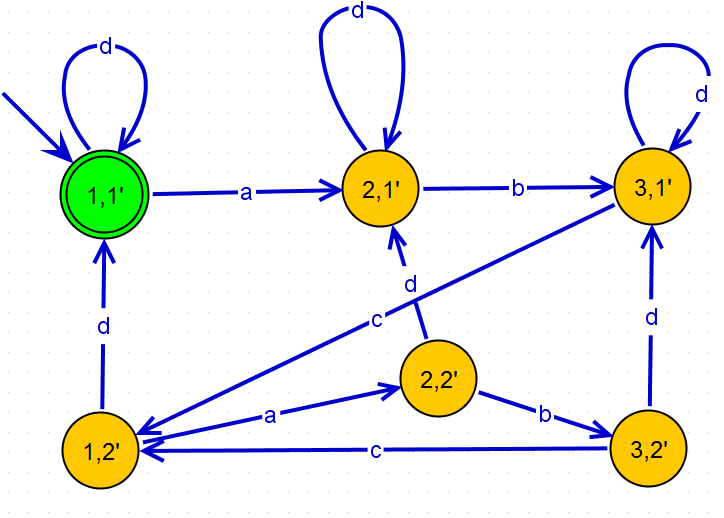
\includegraphics[width = 0.5\textwidth]{./II/images/P.png}
\caption{Modèle de procédé}
\end{figure}

En suivant les consignes de l'objectif, nous avons modélisé notre modèle de spécifications cette manière, \begin{figure}[!ht]
\centering
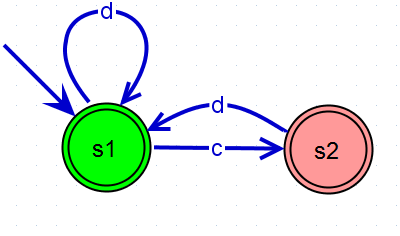
\includegraphics[width = 0.5\textwidth]{./II/images/S.png}
\caption{Modèle des spécifications}
\end{figure}
représenté sur $\Sigma_S = \left\lbrace c,d\right\rbrace$. Nous remarquons que l'ensemble des évènements est strictement inclus dans l'ensemble $\Sigma_{P_o}$, ensemble des évènements observables de $P$, donc notre spécifications est dite partielle. Nous avons de même une représentation de séquence d'évènements autorisées donc notre spécification est dite dynamique.

Notre commande supervisé obtenu avec DESUMA est (produit parallèle):\begin{figure}[!ht]
\centering
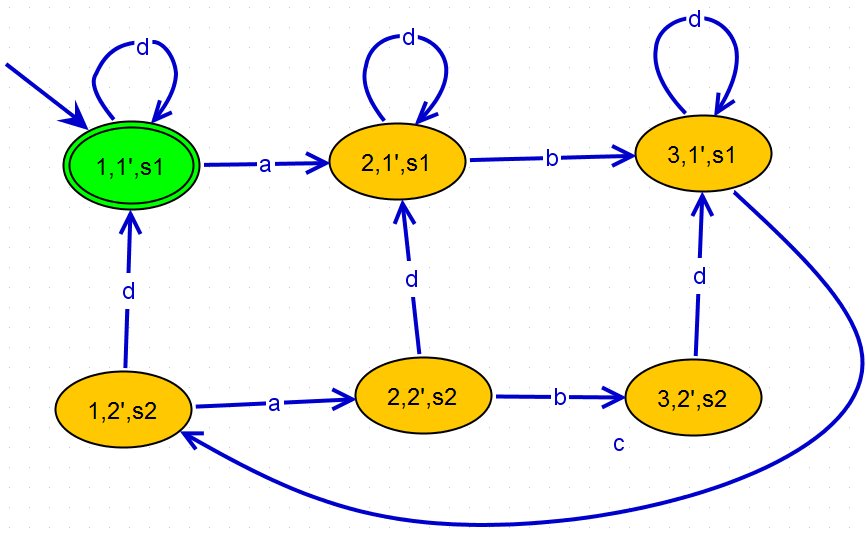
\includegraphics[width = 0.5\textwidth]{./II/images/P_S.png}
\caption{Modèle de commande supervisé}
\end{figure}

L'analyse de DESUMA nous indique que notre modèle n'est pas contrôlable. En effet,  partir de l'état $(3,2)$, il est possible d'avoir une séquence contenant $c$, qui n'est pas contrôlable, qui cause une séquence non souhaitée par les spécifications. C'est pourquoi nous allons maintenant utiliser un algorithme pour rendre P/S contrôlable comme vu pendant nos cours de Diagnostic et Supervision. L'exécution de celui ci est détaillé ci dessous :
\begin{itemize}[label = \textbullet]
\item Nous commençons avec $Q = 0$ et $Q'=0$
\item Vérifions que chaque état ($x_P$,$x_S$) ne contient pas de transition $\delta_S(x_S,\sigma_{nc})\not\in X_S$ et $\delta_P(x_P,\sigma_{nc})\in X_P$ avec $\sigma_{nc}\in\Sigma_{P/S}$ : \\C'est le cas pour la paire ($x_{P_3}$,$x_{S_2}$), on l'ajoute alors à $Q$ : $Q = \left\lbrace (x_{P_3},x_{S_2}) \right\rbrace $
\item Vérifions maintenant qu'aucune séquence non contrôlable de peut amener à une des paires de $Q$ :\\
$\exists s_{nc}$ / $\delta*(x_{P_2},x_{S_2}) \in Q$, alors $Q' = Q\ U\ \left\lbrace x_{P_3},x_{S_2}\right\rbrace$
\item Finalement, nous obtenons : $X_{P/S} = X_{P/S} \backslash \left\lbrace (x_{P_3},x_{S_2}),(x_{P_2},x_{S_2}) \right\rbrace$.
\end{itemize}
\newpage
En enlevant les deux paires (3,2) et (2,2), nous permettons à notre commande supervisé d'être contrôlable. En utilisant cette conclusion, nous obtenons notre commande supervisé contrôlable décrite par le modèle de gauche. Il est cependant possible d'utiliser l'outil de $Controlability$ de DESUMA pour calculer cet automate. Nous le décrivons sur la figure de droite.\begin{figure}[!ht]
\begin{minipage}{.5\textwidth}
\centering
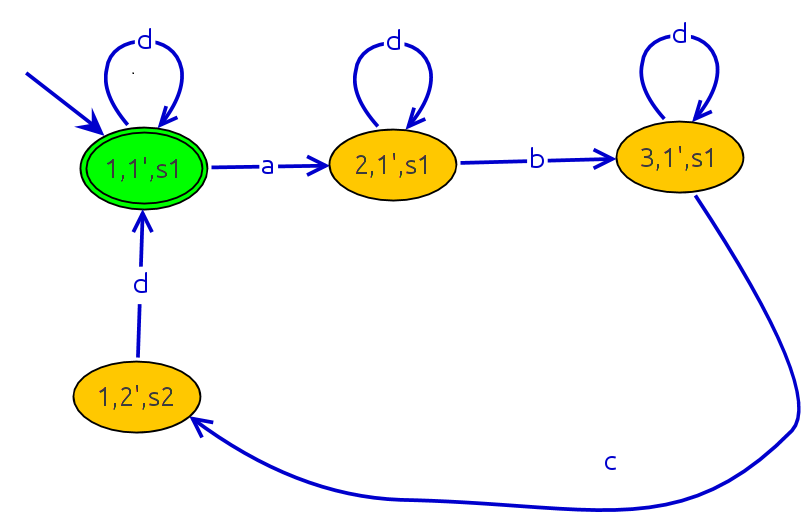
\includegraphics[width=\textwidth]{./II/images/P_S_automate_ctrb_manuel.png}
\caption{Bouchon}
\end{minipage} \hfill
\begin{minipage}{.5\textwidth}
\centering
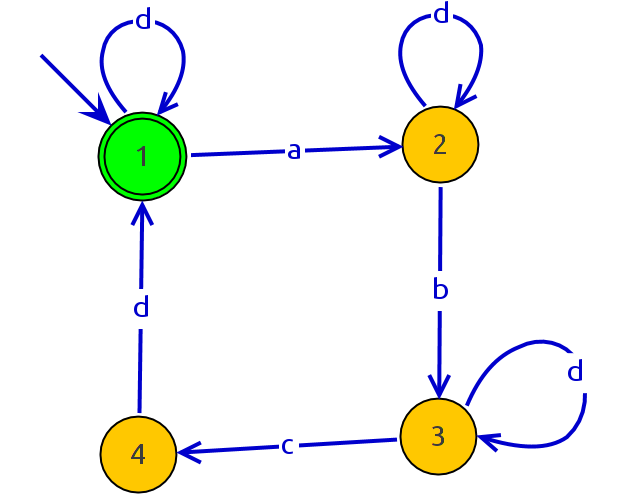
\includegraphics[width=\textwidth]{./II/images/P_S_automate_ctrb_desuma.png}
\caption{Bouteille}
\end{minipage}
\end{figure}


Cependant, cette propriété ne garantit pas le non blocage de notre nouvel automate. A partir de l'état marqué $(1,1')$, nous remarquons que pour chaque état il existe une séquence permettant d'accéder à l'état marqué. Notre commande supervisé est co-accessible et donc non bloquante.